\newpage
\section{Energia}
\subsection{Energia cinetica}
Definiamo \textbf{energia cinetica} di un punto materiale come:
$$K(t) = \frac{1}{2}m||\dot{\vec{r}}(t)||^2 \hspace{15pt} [k] = kg \cdot m^2/s^2 \equiv J \text{"Joule"}$$
La parte di $\frac{1}{2}$ sta per convenzione/comodità, le prime definizioni nel 900 infatti non lo aveva.
\begin{example}
    $\vec{r}(t) = v_0 \cap{x} \hspace{15pt} k= \frac{1}{2}mv_0^2$
\end{example}
\hspace{-15pt}Definiamo \textbf{lavoro} di una forza $\vec{F}(t)$ applicata nella posizione $\vec{r}(t)$ per $t_0 \leq t \leq t_1$
$$L(t_0, t_1) = \int_{t_0}^{t_1}dt \vec{F}(t) \cdot \dot{\vec{r}}(t) \hspace{15pt} [L] = s \cdot N \cdot \frac{m}{s} = J$$
\begin{example}
    $\vec{r} = v_0 \hat{x} \hspace{15pt} \vec{F}(t) = \alpha t \hat{x} + \beta \hat{y} \hspace{15pt} L(t_0, t_1) = \int_{t_0}^{t_1} dt(\alpha t\hat{x} + \beta \hat{y}) \cdot v_0 \hat{x} = \alpha v_0 \frac{t_1^2 - t_0^2}{2}$
\end{example}
$$L(t_0, t_1) = \vec{F}(t) \cdot \vec{d}_{t_0, t_1} \cdot \cos(\Theta) \:\:\: \text{con} \:\:\vec{d}_{t_0, t_1}\:\:\text{spospamento dell'oggetto}$$
\begin{theorem}[Delle forze vive]
    Per un punto materiale, la variazione di energia cinetica è pari al lavoro delle forze.
    $$K(t_1) - K(t_0) = L_1(t_0, t_1) + L_2(t_0, t_1) + \dots$$
\end{theorem}
\hspace{-15pt}Segue dalla seconda legge di Newton:
\begin{equation*}
    \begin{split}
        \sum_{i} d\alpha_i(t) & = \sum_i dt \cdot \vec{F}(t) \cdot \dot{\vec{r}}(t) = dt (\sum_i \vec{F_1}(t)) \cdot \dot{\vec{r}}(t)\\
                              & = dt \cdot m \ddot{\vec{r}}(t) \cdot \dot{\vec{r}}(t) = dt \cdot m \cdot \frac{1}{2}\frac{d}{dt}||\dot{\vec{r}}(t)||^2\\
                              & = \frac{1}{2}md||\dot{\vec{r}}(t)||^2 \:\: \text{e integro membro a membro.}
    \end{split}
\end{equation*}
Se la forza dipende solo dalla posizione di applicazione $\vec{r}(t)$, ma non esplicitamente dal tempo t, si dice \textbf{posizionale}. Questo vuol
dire che, se immaginiamo un punto materiale che fa un determianta legge oraria, man mano che il punto materiale si muove il suo valore cambia, ed anche la forza 
cambia, quindi cambia in base alla posizione.
\begin{example}
    $\vec{F}(\vec{r}(t)) = \vec{F}(x(t), y(t)) = \alpha x(t) \hat{x} + \beta y(t) \hat{y}$
\end{example}
\hspace{-15pt}La dipendenza dal tempo è determinata dall'eventuale movimento della posizione di applicazione. È ben definita $\vec{F}(\vec{r}) \forall t$. \\\\
Per una forza posizione il lavoro si semplifica e diventa:
\begin{equation*}
    \begin{split}
        L(t_0, t_1) & = \int_{t_0}^{t_1}dt \vec{F}(t) \cdot \dot{\vec{r}}(t) = \int_{t_0}^{t_1}dt \vec{F}(\vec{r}(t)) \cdot \dot{\vec{r}}(t) \\
                    & = \sum_i \Delta t_i \vec{F}(\vec{r_i}) \cdot \frac{\vec{r_{i+1}} - \vec{r_i}}{\Delta t_i} = \int_{\vec{r}(t_0 )}^{\vec{r}(t_i)} d\vec{r}\cdot \vec{F}(\vec{r}) = L_e \:\:\text{"integrale di lena"}
    \end{split}
\end{equation*}
Dipende dalla traiettoria, non dalla legge oraria.
\begin{figure}[h!]
    \centering
    \begin{subfigure}{0.3\textwidth}
        \centering
        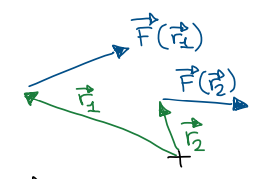
\includegraphics[width=\textwidth]{images/ess-energia1.png}
    \end{subfigure}
    \hspace{15pt}
    \begin{subfigure}{0.4\textwidth}
        \centering
        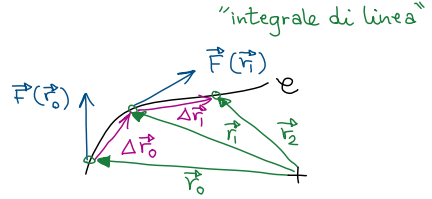
\includegraphics[width=\textwidth]{images/ess-energia-2.png}
    \end{subfigure}
\end{figure}
\begin{example}
    $\vec{F}(x)= -kx\hat{x} \hspace{20pt} \vec{r}(t) = v_0 \cdot \cos(\Omega t)\hat{x}$\\
    $t_0 = 0, \vec{r}(t_0) = x_0 \hat{x}, \hspace{15pt} t_1 = \frac{\pi}{\Omega}, \hspace{15pt} \vec{r}(t_1) = x_0 \cdot (-1)\hat{x}$\\
    $L(t_0, t_1) = \int_{x_0}^{-x_0}dx \hat{x} \cdot (-kx\hat{x}) = -k \frac{x^2}{2} |_{x_0}^{-x_0} = -k x_0^2 \:\: \text{non dipende da }\Omega$
\end{example}
% DA CORREGGERE seguendo nuovo pdf
\begin{observation}
    Per calcolare l'integrale di linea può comunque convenire la formula $\int_{t_0}^{t_1}dt \vec{F}(\vec{r}(t))$. 
    $\dot{\vec{r}}(t)$ eventualmente usando una legge oraria più semplice con medesima traiettoria.
\end{observation}
\begin{example}
    $\vec{F}(\vec{r}) = -kx\hat{x} \hspace{15pt}\vec{r}(t) = R\vec{r}, \Theta(t) = \Omega t \Rightarrow x(t) = R \cos(\Omega t)$\\
    $t_0 = 0, \Theta(t_0) = 0, \hspace{10pt}t_1 = \frac{\pi}{2\Omega}, \Theta(t_1) = \frac{\pi}{2} \hspace{10pt} \dots d\vec{r}\dots \hspace{15pt} \dot{\vec{r}}(t) = R\Omega\hat{\Theta} = -R\Omega\sin(\Omega t)\hat{x} + R\Omega \cos(\Omega t)\hat{y}$
    \begin{equation*}
        \begin{split}
            L(t_0, t_1) & = \int_{t_0}^{t_1}dt \vec{F}(\vec{r}(t)) \cdot \dot{\vec{r}}(t) = \int_{0}^{\pi/2\Omega}[-k R \cos(\Omega t)\hat{x}] \cdot [-R \Omega \sin(\Omega t) \hat{x} + R\Omega \cos(\Omega t)\hat{y}]\\
                        & = \int_{0}^{\pi/2\Omega}kR^2 \Omega \frac{1}{2}\sin(2\Omega t \:\: (\equiv \alpha) \:\:) = kR^2 \Omega \frac{1}{2}\int_{0}^{\pi} \frac{d\alpha}{2\Omega}\sin\alpha = \frac{1}{4} kR^2[-\cos\alpha] = \frac{1}{2}kR^2 
        \end{split}
    \end{equation*}
\end{example}
\hspace{-15pt}Se la forza è \textbf{uniforme} lungo il percorso abbiamo
$$L(t_0, t_1) = \vec{F} \cdot \int_{\vec{r}(t_0)}^{\vec{r}(t_1)} = \vec{F} \cdot [\vec{r}(t_1) - \vec{r}(t_0)] \:\text{(spostamento)}$$
\begin{example}
    $\vec{F}(\vec{r}) = \vec{F}(z) = -mg\hat{z}$ (uniforme ovunque).\\
    $\vec{r}(t) = v_0 t\hat{z} \hspace{20pt} t_0 = 0 \vec{r}(t_0) = 0 \hspace{20pt} t_1 = \frac{h}{v_0} \vec{r}(t_1) = h\hat{z} \hspace{20pt}$
    $$L(t_0, t_1) = \int_{0}^{hat}dz \hat{z} \cdot (-mg\hat{z}) = -mgh$$
\end{example}
\hspace{-15pt}Una forza posizione si dice \textbf{conservativa} e il lavoro non dipende dal percorso, ma solo dalle posizioni iniziali e finali.
Questo accade se e solo se esiste una funzione $u(\vec{r})$ detta \textbf{potenziale} tale che:
$$\vec{F}(\vec{r}) = -\vec{\nabla}u(\vec{r}) \equiv (-\frac{d}{dx}u(\vec{r}), -\frac{d}{dy}u(\vec{r}), -\frac{d}{dz}u(\vec{r}))$$
In tal caso $\int_{\vec{r_0}}^{\vec{r_1}} d\vec{r} \cdot \vec{F}(\vec{r}) = u(\vec{r}_0) - u(\vec{r}_1)$
\begin{itemize}
    \item Forza peso: $u(\vec{r}) = mgz \hspace{20pt} \frac{d}{dx}u(\vec{r}) = \frac{d}{dy}u(\vec{r}) = 0 \hspace{10pt} \frac{d}{dz}u(\vec{r}) = mg \Rightarrow \vec{\nabla}u(\vec{r}) = (0,0, mg)= mg\hat{z} \Rightarrow$
    $$ \vec{F}= -mg\hat{z}$$
    \item Oscillatore unidimensionale: $u(\vec{r}) = \frac{1}{2}kx^2 \hspace{20pt} \frac{d}{dy}u(\vec{r}) = \frac{d}{dz} u(\vec{r}) = 0 \hspace{10pt} \frac{d}{dx}u(\vec{r}) = kx \Rightarrow \vec{\nabla}u(\vec{r}) = (kx, 0, 0) = kx\hat{x} \Rightarrow$
    $$ \vec{F} = -kx\hat{x}$$
\end{itemize}
\begin{observation}
    Una forza non posizionale (es. reazioni vincolari) non può essere conservativa.
\end{observation}

\subsection{Energia meccanica}
Il potenziale è definito "a meno di una costante" perché $-\vec{\nabla}[u(\vec{r}) + u_0] = -\vec{\nabla}u(\vec{r})$. Es: $mg(z-z_0)$
Per un punto materiale, la somma di energia cinetica e dei potenziali delle forze (conservative) alle quali è soggetto (calcolati nella sua posizione) si 
dice \textbf{energia meccanica}.
$$E(t) = K(t) + u_1(\vec{r}(t)) + u_2(\vec{r}(t)) + \cdots$$
Dal teorema delle forze vive segue che la variazione di energia meccanica è pari al lavoro delle forze \textbf{non conservatie}
$$E(t_1) - E(t_0) = L_1^{NC}(t_0, t_1) + L_2^{NC}(t_0, t_1) + \cdots \hspace{10pt} \Rightarrow \hspace{10pt} L(t_0, t_1) = E(t_1) - E(t_0)$$
Se $L_i^{NC} = 0$ l'energia meccanica è \textbf{costante} nel tempo ("conservata").
$$E_{mecc} = E_{cin} + E_{pot} \:\:\: \Rightarrow \:\:\: \Delta E_{mecc} = E_{mecc,finale} - E_{mecc, iniziale}$$
Il profilo del potenziale visualizza le forze.
\begin{figure}[h!]
    \centering
    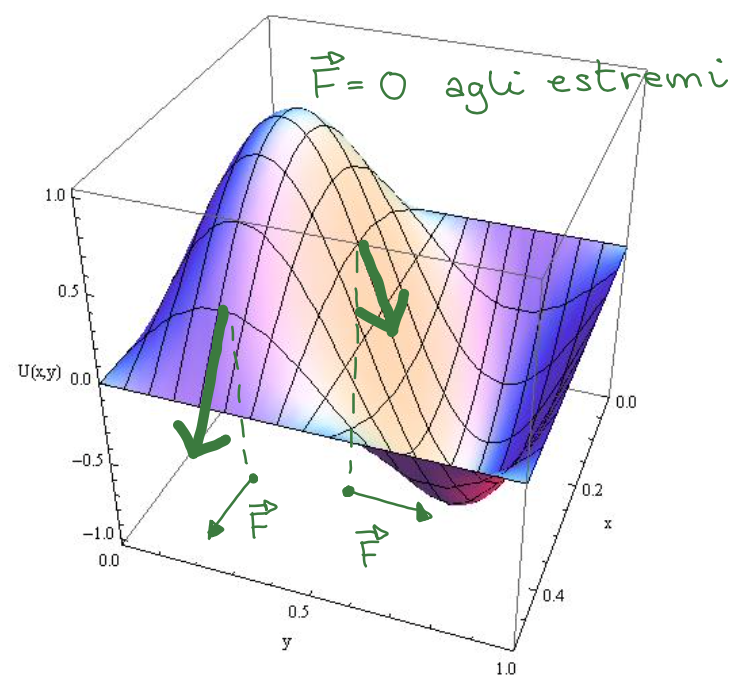
\includegraphics[width=0.28\textwidth]{images/profilo-potenziale.png}
\end{figure}
\newpage
Il profilo di potenziale visualizza le regioni dove il moto è permesso se l'energia è conservata.
\begin{figure}[h!]
    \centering
    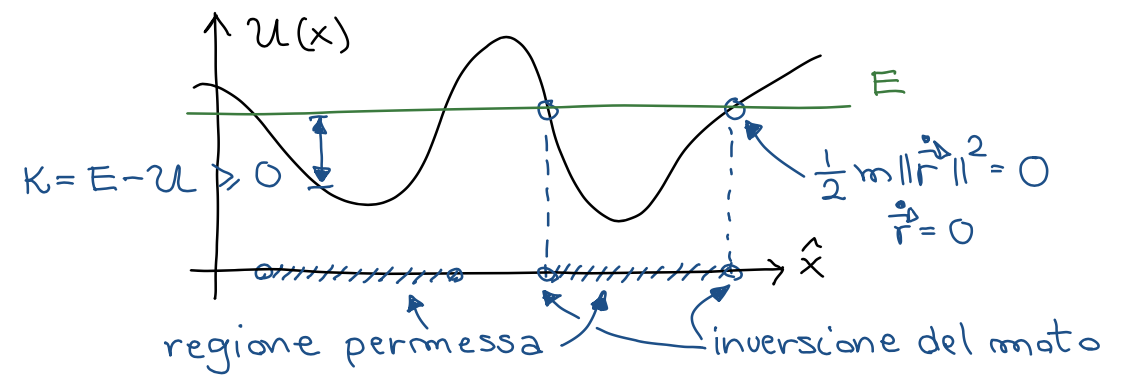
\includegraphics[width=0.75\textwidth]{images/regioni-permesse-profilo-potenziale.png}
\end{figure}
\begin{observation}
    Il "tunneling" tra regioni permesse disgiunte è possibile per atomi e particelli subatomiche secondo
    le leggi della \textbf{meccanica quantistica}.
\end{observation}
